\begin{figure}
\center

	\begin{subfigure}[t]{0.22\textwidth}
		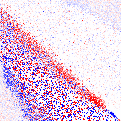
\includegraphics[width=\stratgraphwidth]{images/findings/round1/diff/hand_max_min.png}
		\caption{\handmaxmin}
	\end{subfigure}
	~
	\begin{subfigure}[t]{0.22\textwidth}
		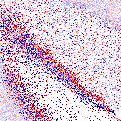
\includegraphics[width=\stratgraphwidth]{images/findings/round1/diff/hand_max_avg.png}
		\caption{\handmaxavg}
	\end{subfigure}
~
	\begin{subfigure}[t]{0.22\textwidth}
		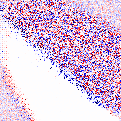
\includegraphics[width=\stratgraphwidth]{images/findings/round1/diff/hand_max_med.png}
		\caption{\handmaxmed}
	\end{subfigure}
	~
	\begin{subfigure}[t]{0.22\textwidth}
		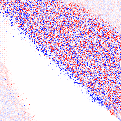
\includegraphics[width=\stratgraphwidth]{images/findings/round1/diff/hand_max_poss.png}
		\caption{\handmaxposs}
	\end{subfigure}

	\begin{subfigure}[t]{0.22\textwidth}
		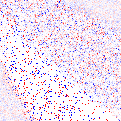
\includegraphics[width=\stratgraphwidth]{images/findings/round1/diff/crib_min_avg.png}
		\caption{\cribminavg}
	\end{subfigure}
	~
	\begin{subfigure}[t]{0.22\textwidth}
		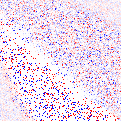
\includegraphics[width=\stratgraphwidth]{images/findings/round1/diff/pegging_max_avg_gained.png}
		\caption{\peggingmaxavggained}
	\end{subfigure}
~
	\begin{subfigure}[t]{0.22\textwidth}
		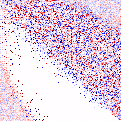
\includegraphics[width=\stratgraphwidth]{images/findings/round1/diff/pegging_max_med_gained.png}
		\caption{\peggingmaxmedgained}
	\end{subfigure}
	~
	\begin{subfigure}[t]{0.22\textwidth}
		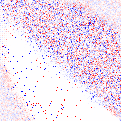
\includegraphics[width=\stratgraphwidth]{images/findings/round1/diff/pegging_min_avg_given.png}
		\caption{\peggingminavggiven}
	\end{subfigure}

\caption{
	Difference graphs for each strategy.
	%
	In these graphs,
	blue spaces represent those score locations
		in which the pone preferred to play by the given strategy
		while the dealer did not,
	and vice versa for red.
	%
	White spaces show locations where the strategy's strength is
	mostly equivalent between the two roles.
}
\label{fig:r1-diff}
\end{figure}

